%%%% ijcai21.tex
%
\typeout{Improved guarantees and a multiple-descent curve for 
  Column Subset Selection 
  and the Nystr\"om method$^*$}

% These are the instructions for authors for IJCAI-21.

\documentclass{article}
\pdfpagewidth=8.5in
\pdfpageheight=11in
% The file ijcai21.sty is NOT the same than previous years'
\usepackage{sty/ijcai2021/ijcai21}

% Use the postscript times font!
\usepackage{natbib}
\usepackage{times}
\usepackage{soul}
\usepackage{url}
\usepackage[hidelinks]{hyperref}
\usepackage[utf8]{inputenc}
\usepackage[small]{caption}
\usepackage{graphicx}
\usepackage{amsmath}
\usepackage{amsthm}
\usepackage{booktabs}
\usepackage{algorithm}
\usepackage{algorithmic}
\usepackage{xcolor}
\usepackage{xfrac}
\usepackage{amssymb}

\urlstyle{same}

% the following package is optional:
%\usepackage{latexsym}

% See https://www.overleaf.com/learn/latex/theorems_and_proofs
% for a nice explanation of how to define new theorems, but keep
% in mind that the amsthm package is already included in this
% template and that you must *not* alter the styling.
\newtheorem{example}{Example}
\newtheorem{theorem}{Theorem}

% Following comment is from ijcai97-submit.tex:
% The preparation of these files was supported by Schlumberger Palo Alto
% Research, AT\&T Bell Laboratories, and Morgan Kaufmann Publishers.
% Shirley Jowell, of Morgan Kaufmann Publishers, and Peter F.
% Patel-Schneider, of AT\&T Bell Laboratories collaborated on their
% preparation.

% These instructions can be modified and used in other conferences as long
% as credit to the authors and supporting agencies is retained, this notice
% is not changed, and further modification or reuse is not restricted.
% Neither Shirley Jowell nor Peter F. Patel-Schneider can be listed as
% contacts for providing assistance without their prior permission.

% To use for other conferences, change references to files and the
% conference appropriate and use other authors, contacts, publishers, and
% organizations.
% Also change the deadline and address for returning papers and the length and
% page charge instructions.
% Put where the files are available in the appropriate places.

%PDF Info Is REQUIRED.
\pdfinfo{
/TemplateVersion (IJCAI.2021.0)
}

\title{Improved Guarantees and a Multiple-descent Curve\\
  for Column Subset Selection 
  and the Nystr\"om Method (Extended Abstract)$^*$}

% Single author syntax
%\author{
%    Zhi-Hua Zhou
%    \affiliations
%    Nanjing University
%    \emails
%    pcchair@ijcai-21.org
%}

% Multiple author syntax (remove the single-author syntax above and the \iffalse ... \fi here)
% Check the ijcai21-multiauthor.tex file for detailed instructions
%\iffalse
\author{
Micha{\l } Derezi\'{n}ski$^{1\dagger}$
\and
{Rajiv Khanna}$^1$\and
Michael W. Mahoney$^{1,2}$
\affiliations
$^1$Department of Statistics,
  University of California at Berkeley\\
$^2$International Computer Science Institute, Berkeley \\
\emails
\{mderezin, rajivak\}@berkeley.edu,
mmahoney@stat.berkeley.edu
}
%\fi
\ifx\definition\undefined
\newtheorem{definition}{Definition}
\fi
\ifx\remark\undefined
\newtheorem{remark}{Remark}
\fi
\ifx\corollary\undefined
\newtheorem{corollary}{Corollary}
\fi
\ifx\lemma\undefined
\newtheorem{lemma}{Lemma}
\fi
\newcommand{\Er}{\mathrm{Er}}
\def\A{\mathbf A}
\def\B{\mathbf B}
\def\C{\mathbf C}
\def\P{\mathbf P}
\def\E{\mathbb E}
\def\R{\mathbb R}
\def\N{\mathbb N}
\def\K{\mathbf K}
\def\I{\mathbf I}
\def\K{\mathbf K}
\def\tr{\mathrm{tr}}
\def\Ot{\widetilde{O}}
\def\Kbh{{\widehat{\K}}}
\def\rank{\mathrm{rank}}
\def\opt{{\textsc{OPT}_k}}
\def\a{\mathbf a}
\def\DPP{{\mathrm{DPP}}}
\def\sr{{\mathrm{sr}}}
\def\Nc{\mathcal{N}}


\begin{document}

\maketitle

\begin{abstract}
 The Column Subset Selection Problem (CSSP) and the Nystr\"om method
are among the leading tools for constructing interpretable low-rank
approximations of large datasets by selecting a small but
representative set of features or instances. 
A fundamental question in this area is: what is the cost of this
interpretability, i.e., how well can a data subset of
size $k$ compete with the best rank $k$ approximation?
We develop techniques which exploit spectral properties of the data
matrix to obtain improved approximation guarantees which go beyond the
standard worst-case analysis.
Our approach leads to significantly better bounds for datasets with
known rates of singular value decay, e.g., polynomial or exponential
decay.
Our analysis also reveals an intriguing phenomenon: the cost of
interpretability as a function of $k$ may exhibit multiple peaks and
valleys, which we call a multiple-descent curve.
A lower bound we establish shows that this behavior is not an artifact
of our analysis, but rather it is an inherent property of the CSSP and
Nystr\"om tasks.
Finally, using the example of a radial basis function (RBF)
kernel, we show that both our improved bounds and the multiple-descent
curve can be observed on real datasets simply by varying the
RBF~parameter.
\end{abstract}
\section{Introduction}
\label{s:intro}

{\renewcommand{\thefootnote}{\fnsymbol{footnote}}
\footnotetext[1]{This is an abridged version invited to IJCAI 2021 of a
  longer paper with the same title that appeared in NeurIPS 2020 and
  received a Best Paper Award.}
  \footnotetext[2]{Corresponding author.}}

We consider the task of selecting a small but representative sample of
column vectors from a large matrix. Known as the \emph{Column Subset Selection
Problem} (CSSP), this is a well-studied combinatorial optimization task with
many applications in machine learning. %  
%\citep[e.g., feature selection, see][]{Guyon03FeatureSelection,BoutsidisMD08},
%scientific computing \citep[e.g.,][]{Chan92RankRevealingQR,Drineas08CUR} and signal processing
%\citep[e.g.,][]{Balzano10MatchedSubspace}. 
In a 
commonly studied variant of this task, we aim to minimize the
squared error of projecting all columns of the matrix onto the
subspace spanned by the chosen column subset.
\begin{definition}[CSSP]
  Given an $m\times n$ matrix $\A$, pick a set $S\subseteq\{1,...,n\}$ of 
  $k$ column indices, to minimize
  \begin{align*}
   \Er_\A(S) := \|\A - \P_S\A\|_F^2,
  \end{align*}
  where $\|\cdot\|_F$ is the Frobenius norm, $\P_S$ is the
  projection onto $\mathrm{span}\{\a_i:i\in S\}$ and $\a_i$ denotes the $i$th
  column of~$\A$.
\end{definition}
Another variant of the CSSP emerges in the kernel
setting under the name \emph{Nystr\"om method}
\citep{Williams01Nystrom,dm_kernel_JRNL,revisiting-nystrom}. We also
discuss this variant, showing how our analysis applies in this context.
Both the CSSP and the Nystr\"om method are ways of
constructing accurate low-rank approximations by using submatrices of
the target matrix. Therefore, it is natural to ask how
close we can get to the best possible rank~$k$ approximation error:
\begin{align*}
  \opt := \!\!\min_{\B:\,\rank(\B)=k} \!\!\|\A-\B\|_F^2\leq \min_{S:\,|S|=k}\Er_\A(S).
\end{align*}

While the best possible rank $k$ approximation has the lowest
approximation error, the approximated matrix $\B$ is not
{input-sparse}. As such, it is not \emph{interpretable} since a
practitioner is unable to attribute the quality of approximation to
specific physical quantities represented by the columns of the
matrix~$\A$ \citep{mahoney2009cur}. Such \emph{interpretable}
dimensionality reduction is desirable 
in many machine learning applications. 
 Our goal is to find a subset $S$ of size $k$ for which the cost of
 interpretability is small, as measured by what we call the
 \emph{approximation factor}: the ratio
between $\Er_\A(S)$ and $\opt$. Furthermore, a brute force
search requires iterating over all 
${n \choose k}$ subsets, which is prohibitively expensive, so we
would like to find our subset more efficiently.

\begin{figure}
%\begin{wrapfigure}{r}{0.45\textwidth}
 % \vspace{-5mm}
  %\fi
  \centering  
  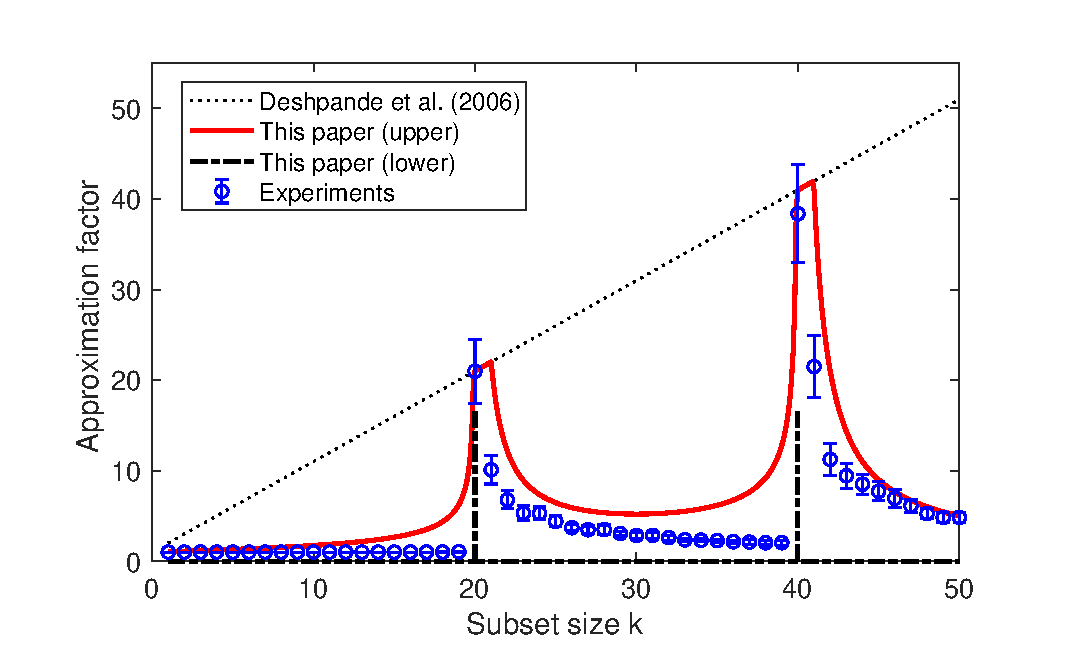
\includegraphics[width=0.47\textwidth]{figs/nystrom/nystrom-bounds}
  \caption{Empirical study of the
    expected approximation factor $\E[\Er_\A(S)]/\opt$ for
a $k$-DPP with
    different subset sizes $|S|=k$, compared to our theory. We use a
    data matrix $\A$ 
    whose
    spectrum exhibits two sharp drops, demonstrating
multiple-descent. The lower bounds are based on Theorem
    \ref{t:lower}, whereas, as our upper bound, we plot the
    minimum over all $\Phi_s(k)$ from
    Theorem~\ref{t:upper}. Note that multiple-descent vanishes under
    smooth spectral decay, resulting in improved guarantees (see
    Theorem \ref{t:decay}).
  }
  \label{f:intro}
  \end{figure}
%  \else
%  \end{wrapfigure}\fi

In terms of worst-case analysis, 
\citet{pca-volume-sampling} gave a randomized
method 
which returns a
set $S$ of size $k$ such that: %\vspace{-4mm}
\begin{align}
  \frac{\E[\Er_\A(S)]}{\opt}\leq k+1.\label{eq:old-bound}
\end{align}
While the original algorithm was slow, 
efficient implementations have been provided since then
\citep[e.g., see][]{efficient-volume-sampling,dpp-intermediate}.
The method belongs to the family of cardinality constrained
Determinantal Point Processes \citep[DPPs, see][]{dpps-in-randnla}, and will
be denoted as $S\sim k\text{-}\DPP(\A^\top\A)$. 
The approximation  factor  $k+1$ is optimal in the worst-case,
since for any $0<k<n\leq m$ and $0<\delta<1$, an $m\times n$
matrix~$\A$ can be constructed for which $\frac{\Er_{\A}(S)}{\opt}\geq
(1-\delta)(k+1)$ for all subsets $S$ of size $k$. 
Yet it is known that, in practice, CSSP algorithms perform better
than worst-case, so the question we consider is: how can we go beyond
the usual worst-case analysis to accurately reflect what is possible
in the CSSP?  

\textbf{Contributions.} We provide improved guarantees for the CSSP
approximation factor, which go beyond the worst-case analysis and 
which lead to surprising conclusions.%\vspace{-3mm}
\begin{enumerate}
\item\underline{New upper bounds}:
We develop a family of upper bounds on the CSSP approximation factor
(Theorem~\ref{t:upper}), which we call the Master Theorem
as they can be used to derive a number 
of new guarantees. In particular, we show that when the data matrix $\A$ exhibits a
known spectral decay, then \eqref{eq:old-bound} can often be
drastically improved (Theorem \ref{t:decay}).
\item \underline{New lower bound}:
Even though the worst-case upper bound in \eqref{eq:old-bound} can often
be loose, there are cases when it cannot be improved.
We give a new lower bound construction (Theorem \ref{t:lower}) showing
that there are matrices $\A$ for which multiple different subset sizes exhibit
worst-case behavior.
\item \underline{Multiple-descent curve}: 
Our upper and lower bounds
reveal that for some matrices the CSSP approximation factor can exhibit
peaks and valleys as a function of the subset size $k$ (see Figure
\ref{f:intro}).  We show that this phenomenon is an inherent property
of the CSSP  (Corollary \ref{c:multiple-descent}).
\end{enumerate}



\section{Determinantal Point Processes}
\label{s:dpp}

Since our main results rely on randomized subset selection via
determinantal point processes (DPPs), we provide a brief overview of
the relevant aspects of this class of distributions.
First introduced by \citet{Macchi1975}, a determinantal point process is a
probability distribution over subsets $S \subseteq[n]$, where we use $[n]$
to denote the set $\{1,...,n\}$. The relative probability of a subset being drawn is 
governed by a positive semidefinite (p.s.d.) matrix $\K \in \R^{n\times n}$,
as stated in the definition below, where we use $\K_{S,S}$ to denote
the $|S|\times |S|$ submatrix of $\K$ with rows and columns indexed
by $S$.
\begin{definition}\label{d:dpp}
  For an $n\times n$ p.s.d.~matrix $\K$, define $S\sim
  \DPP(\K)$ as a distribution 
  over all subsets $S\subseteq [n]$ so
  that
  \[\Pr(S)=\frac{\det(\K_{S,S})}{\det(\I+\K)}.\]
A restriction to subsets of size $k$ is denoted as $k$-$\DPP(\K)$.
\end{definition}
DPPs can be used to introduce diversity in the selected set or to
model the preference for selecting dissimilar items, where the
similarity is stated by the kernel matrix $\K$. DPPs are
commonly used in many machine learning applications where these
properties are desired, e.g.,~recommender systems~\citep{Warlop2019}, model
interpretation~\citep{kim:2016MMD}, text
and video summarization~\citep{dpp-video}, and others
\citep{dpp-ml}. For a recent survey, see \cite{dpps-in-randnla}.

Given a p.s.d.~matrix $\K \in \R^{n \times n}$ with eigenvalues
$\lambda_1,...\, \lambda_n$, the size of the set $S \sim \DPP(\K)$
is distributed as a Poisson binomial random variable, namely, the
number of successes in $n$ Bernoulli random trials where the
probability of success in the $i$th trial is given by 
$\frac{\lambda_i}{\lambda_i+1}$. This leads to a simple
expression for the expected subset size:
\begin{align}
\E[|S|] = \sum_i \frac{\lambda_i}{\lambda_i + 1} = \tr(\K(\I + \K)^{-1}).\label{eq:size}
\end{align}
Note that if $S\sim\DPP(\frac1\alpha\K)$, where $\alpha>0$, then
$\Pr(S)$ is proportional to $\alpha^{-|S|}\det(\K_{S,S})$, so rescaling the kernel
by a scalar only affects the distribution of the subset sizes, giving
us a way to set the expected size to a desired value (larger $\alpha$
means smaller expected size).
Nevertheless, it is still often preferrable to restrict the size of
$S$ to a fixed $k$, obtaining a $k$-$\DPP(\K)$ \citep{k-dpp}.

Both DPPs and $k$-DPPs can be sampled efficiently, with some of the
first algorithms provided by
\citet{dpp-independence},
\citet{efficient-volume-sampling}, \citet{k-dpp} and others. These
approaches rely on an eigendecomposition of the kernel $\K$, at the cost of $O(n^3)$. When
$\K=\A^\top\A$, as in the CSSP, and the dimensions satisfy $m\ll n$, then this can be improved
to $O(nm^2)$. More recently, algorithms that avoid computing the
eigendecomposition have been proposed
\citep{dpp-intermediate,dpp-sublinear,alpha-dpp,rayleigh-mcmc},
resulting in running times of $\Ot(n)$ when given matrix $\K$ and
$\Ot(nm)$ for matrix $\A$, assuming small desired subset size.
See \citet{dppy} for an efficient Python implementation of DPP sampling.

The key property of DPPs that enables our analysis is a
formula for the expected value of the random matrix that is the orthogonal projection onto the
subspace spanned by vectors selected by $\DPP(\A^\top\A)$.
In the special case when $\A$ is a square full rank matrix, the
following result can be derived as a corollary of Theorem 1 by
\citet{randomized-newton}, and a variant for DPPs over
continuous domains can be found as Lemma~8 of
\citet{surrogate-design}. 
\begin{lemma}\label{l:expectation_proj}
  For any $\A$ and $S\subseteq [n]$, let $\P_S$ be the  
projection onto the $\mathrm{span}\{\a_i:i\in S\}$. If $S\sim \DPP(\A^\top\A)$, then
\begin{align*}
  \E[\P_S] & = \A(\I+\A^\top\A)^{-1}\A^\top.
\end{align*}
\end{lemma}
Lemma~\ref{l:expectation_proj} implies a simple closed form expression for
the expected error in the CSSP presented next. Here, we use a
rescaling parameter $\alpha>0$ for controlling
the distribution of the subset sizes. Note that it is crucial that we
are using a DPP with random subset size, because the corresponding
expression for the expected error of the fixed size $k$-DPP is
combinatorial, and therefore much harder to work with.
\begin{lemma}\label{l:expected-error}
  For any $\alpha>0$, if $S\sim
  \DPP(\frac1\alpha\A^\top\A)$, then
  \begin{align*}
    \E\big[\Er_\A(S)\big] =
    \tr\big(\A\A^\top(\I+\tfrac1\alpha\A\A^\top)^{-1}\big) = \E[|S|]\cdot\alpha.
  \end{align*}
\end{lemma}

\section{Main Results}
Our upper bounds rely on the notion of effective dimensionality called
stable rank~\citep{ridge-leverage-scores}. Here, we use an extended version of this concept, as
defined by \citet{BLLT19_TR}.
\begin{definition}[Stable rank]
Let $\lambda_1\geq \lambda_2\geq ...$ denote the eigenvalues of the
matrix $\A^\top\A$. For  $0\leq s<\rank(\A)$, we define the stable
rank of order $s$ as $\sr_s(\A) = \lambda_{s+1}^{-1}\sum_{i>s}\lambda_i$.
\end{definition}
In the following result, we define a family of functions $\Phi_s(k)$ which
bound the approximation factor $\Er_\A(S)/\opt$ in the range of $k$ between $s$ and
$s+\sr_s(\A)$. We call this the Master Theorem because we use it to derive
a number of more specific upper bounds.
\begin{theorem}[Master Theorem]\label{t:upper}
Given $0\leq s<\rank(\A) $, let  $t_s = s+\sr_s(\A)$,
and suppose that $s+ \frac7{\epsilon^4}\ln^2\!\frac1\epsilon \leq k\leq t_s-1$,
where $0<\epsilon\leq\frac12$. If $S\sim k$-$\DPP(\A^\top\A)$, then
\begin{align*}
  &\frac{\E[\Er_\A(S)]}{\opt}\leq (1+2\epsilon)^2\,\Phi_{s}(k),\\
  \text{where }& \Phi_s(k)=\big(1+\tfrac{s}{k-s}\big)\sqrt{1 + \tfrac{2(k-s)}{t_s-k}\,}.
\end{align*}
\end{theorem}
Note that we separated out the dependence on $\epsilon$ from the function
$\Phi_s(k)$, because the term $(1+2\epsilon)^2$ is an artifact of a
concentration of measure analysis that is unlikely to be of practical
significance. We conjecture that the dependence on $\epsilon$
can be eliminated from the statement entirely.% (see Conjecture \ref{c:convex}). 

We next examine the consequences of
the Master Theorem, starting with a sharp transition that occurs as $k$
approaches the stable rank of $\A$. 
\begin{remark}[Sharp transition]\label{r:phase-transition}
For any $k$ it is true that:
%  \vspace{-3mm}
  \begin{enumerate}
\item  For all $\A$, if $k\leq \sr_0(\A)\!-\!1$, then there is a subset $S$ of size $k$ such that
$\frac{\Er_\A(S)}{\opt} = O(\sqrt  k\,)$.
\item There is $\A$ such that $\sr_0(\A)\!-\!1<k<\sr_0(\A)$ and for
  every size $k$ subset $S$, $\frac{\Er_\A(S)}{\opt}
  \geq 0.9\,k$.
  \end{enumerate}
\end{remark}
Part 1 of Remark \ref{r:phase-transition} follows from the Master Theorem by setting
$s=0$, whereas part 2 follows from the lower bound of
\citet{more-efficient-volume-sampling}. Observe how the worst-case
approximation factor jumps from $O(\sqrt k\,)$ to $\Omega(k)$, as $k$
approaches $\sr_0(\A)$. An example of this sharp
transition is shown in Figure \ref{f:intro}, where the stable
rank of $\A$ is around $20$. 

While certain matrices directly exhibit the sharp transition from
Remark \ref{r:phase-transition}, many do not. In particular, for
matrices with a known rate of spectral decay, the Master Theorem can
be used to provide improved guarantees on the CSSP approximation
factor over \emph{all} subset sizes. 

To illustrate this, we give novel bounds
for the two most commonly studied decay rates:  polynomial and exponential.
\begin{theorem}[Examples without sharp transition]\label{t:decay}
Let $\lambda_1\!\geq\!\lambda_2\!\geq\!...$ be the
eigenvalues of $\A^\top\A$. There is an absolute constant $c$ such that
for any $0\!<\!c_1\!\leq\!c_2$, with $\gamma=c_2/c_1$, if:\\[2mm]
\textnormal{1.} (\textbf{polynomial spectral decay}) $c_1i^{-p}\!\leq\!
  \lambda_i\!\leq\! c_2i^{-p}$ for all $i$, with $p>1$, then $S\sim
k$-$\DPP(\A^\top\A)$ satisfies
  \begin{align*}
    \frac{\E[\Er_\A(S)]}{\opt}\leq c \gamma p. 
  \end{align*}
\textnormal{2.} (\textbf{exponential spectral decay}) $c_1(1\!-\!\delta)^{i}\leq \lambda_i\leq
  c_2(1\!-\!\delta)^{i}$ for all $i$, with $\delta\in(0,1)$, then $S\sim
k$-$\DPP(\A^\top\A)$ satisfies %\vspace{-4mm}
  \begin{align*}
    \frac{\E[\Er_\A(S)]}{\opt}\leq c\gamma(1+ \delta k).
  \end{align*}
\end{theorem}
Note that for polynomial decay, unlike in \eqref{eq:old-bound}, the
approximation factor is constant, i.e., it does not depend on $k$. For
exponential decay, our bound provides an improvement over
\eqref{eq:old-bound} when $\delta=o(1)$.
To illustrate how these types of bounds can be obtained from the
Master Theorem, consider the function $\Phi_s(k)$ for some
$s>0$. The first term in the function, $1+\frac{s}{k-s}$, decreases with $k$, whereas
the second term (the square root) increases, albeit at a slower rate. This creates a
U-shaped curve which, if sufficiently wide, has a valley where the
approximation factor can get arbitrarily close to 1. This will occur
when $\sr_s(\A)$ is large, i.e., when the spectrum of $\A^\top\A$ has
a relatively flat region after the $s$th eigenvalue (Figure \ref{f:intro}
for $k$ between 20 and 40). Note that a peak value of some function
$\Phi_{s_1}$ may coincide with a valley of some $\Phi_{s_2}$, so only
taking a minimum over all functions reveals the true approximation
landscape predicted by the Master Theorem. 

The peaks and valleys of the CSSP approximation
factor suggested by Theorem \ref{t:upper} are in fact an
inherent property of the problem, rather than an artifact of our
analysis or the result of using a particular algorithm. We prove this by
constructing a family of matrices $\A$ for which the best possible approximation
factor is large, i.e., close to the worst-case upper bound of
\citet{pca-volume-sampling}, not just for one size $k$, but for a
sequence of increasing sizes.
 \begin{theorem}[Lower bound]\label{t:lower}
For any $\delta\in(0,1)$ and
$0\!=\!k_0\!<\!k_1\!<\!...\!<\!k_t\!<\!n\leq m$, there is a matrix 
$\A\in\R^{m\times n}$ such that for any subset $S$ of size $k_i$,
where $i\in\{1,...,t\}$,
\begin{align*}
\frac{\Er_{\A}(S)}{\textsc{OPT}_{k_i}}\geq (1-\delta)(k_i-k_{i-1}).
  \end{align*}
\end{theorem}
Combining the Master Theorem with the lower
bound of Theorem \ref{t:lower} we can easily provide an example matrix
for which the optimal solution to the CSSP problem exhibits multiple
peaks and valleys. We refer to this phenomenon as the multiple-descent curve.
\begin{corollary}[Multiple-descent curve]\label{c:multiple-descent}
  For $t\in\N$ and $\delta\in(0,1)$, there is a
  sequence $0<k_1^l<k_1^u<k_2^l<k_2^u<...<k_t^l<k_t^u$ and
  $\A\in\R^{m\times n}$ such that for any $i\in\{1,...,t\}$:
  \begin{align*}
    \min_{S:|S|=k_i^l}\frac{\Er_\A(S)}{\textsc{OPT}_{k_i^l}}\leq 1+\delta,
                                 \qquad\text{and } \\
    \min_{S:|S|=k_i^u}\frac{\Er_\A(S)}{\textsc{OPT}_{k_i^u}} \geq
    (1-\delta)(k_i^u+1).
  \end{align*}
\end{corollary}


  \paragraph{The Nystr\"om method.} 
  We briefly discuss how our results translate to guarantees for the Nystr\"om
  mehod, a variant of the CSSP in the kernel setting which has
  gained considerable interest in the machine learning literature~\citep{dm_kernel_JRNL,revisiting-nystrom}.
In this context, rather than being given the column vectors
explicitly, we consider the 
$n\times n$ matrix $\K$ whose entry $(i,j)$ is the dot product
between the $i$th and $j$th vector in the kernel space,
$\langle\a_i,\a_j\rangle_\text{K}$. A Nystr\"om approximation of $\K$ based on subset $S$
is defined as $\Kbh(S) = \C\B^{\dagger}\C^\top$, where $\B$ is the
$|S|\times |S|$ submatrix of $\K$ indexed by $S$, whereas $\C$ is the
$n\times |S|$  submatrix with columns indexed by $S$. 
\begin{remark}
  If $\K=\A^\top\A$ and $\|\cdot\|_*$ is the trace norm, then
    $\big\|\K-\Kbh(S)\big\|_* = \Er_{\A}(S)$ for all $S\subseteq\{1,...,n\}$.
Moreover, the trace norm error of the best rank $k$ approximation of
$\K$, 
is equal to the squared Frobenius norm error of the 
best rank $k$ approximation of $\A$, i.e.,
\[\min_{\Kbh:\,\rank(\K)=k}\|\K-\Kbh\|_* = \opt.\]
\end{remark}

\section{Empirical Evaluation}
\label{s:experiments}


In this section, we provide an empirical evaluation designed to demonstrate how our improved guarantees for the CSSP and Nystr\"om method, as well as the multiple-descent phenomenon, can be easily observed on real datasets. 
We use a standard experimental setup for data subset selection using
the Nystr\"om method \citep{revisiting-nystrom}, where an $n\times n$
kernel matrix $\K$ for a dataset of size $n$ is defined so that the
entry $(i,j)$ is computed using the Gaussian Radial Basis Function  (RBF)
kernel:
$\langle\a_i,\a_j\rangle_\text{K}=\exp(-\|\a_i\!-\!\a_j\|^2/\sigma^2)$,
where $\sigma$ is a free parameter. 
We are particularly interested in the effect of varying $\sigma$.
Nystr\"om subset selection is performed using $S\sim k$-$\DPP(\K)$
(Definition \ref{d:dpp}), and we plot the expected approximation
factor $\E[\|\K-\Kbh(S)\|_*]/\opt$ (averaged over 1000 runs), where
$\Kbh(S)$ is the Nystr\"om approximation of $\K$ based on the subset
$S$, $\|\cdot\|_*$ is the trace norm,
and $\opt$ is the trace norm error of the best rank $k$
approximation. 
This task is
equivalent to the CSSP task defined on the matrix $\A$ such that
$\K=\A^\top\A$. 

\begin{figure}[t]
   \centering
  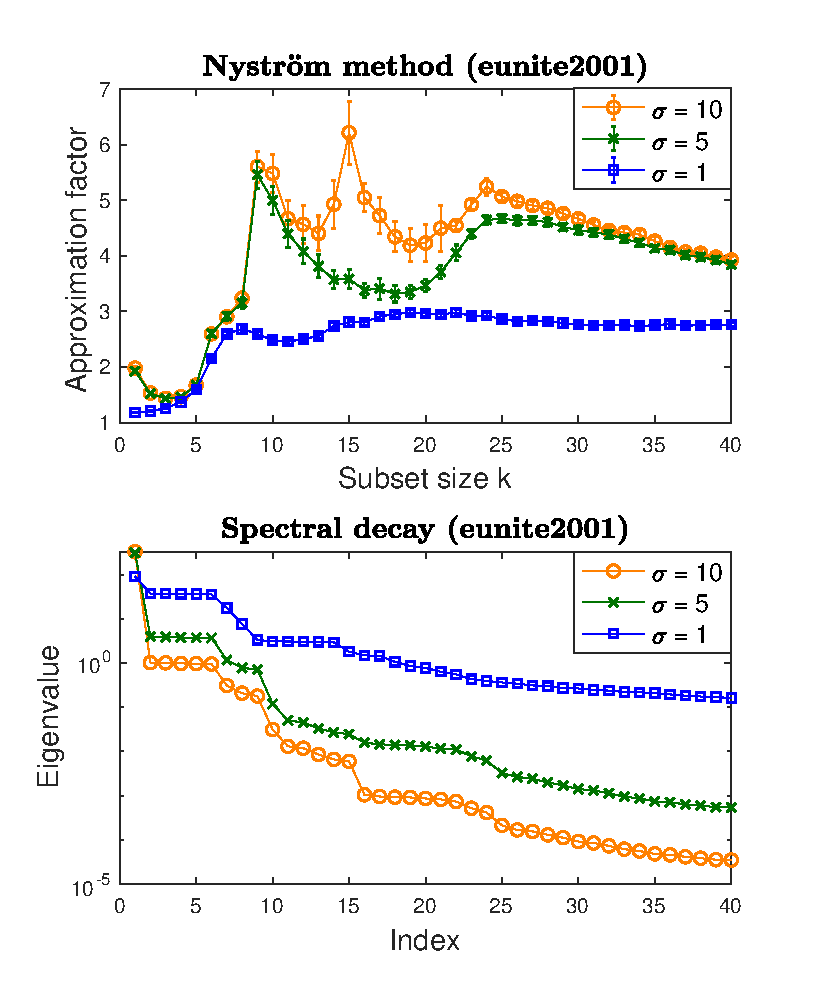
\includegraphics[width=0.45\textwidth]{figs/nystrom/rbf-eunite2001-double}

  \caption{Top plot shows the Nystr\"om approximation factor $\E[\|\K-\Kbh(S)\|_*]/\opt$,
    where $S\sim k$-$\DPP(\K)$ for the eunite2001 Libsvm dataset ($\sigma$ is the RBF parameter). Error bars show three times the standard
    error  of the mean over 1000 trials. Bottom plot shows the spectral decay for  the
  top $40$ eigenvalues of the kernel $\K$. Note that the
  peaks in the approximation factor align with the drops in
  the spectrum.}
  \label{f:rbf}
\end{figure}



The aim of our empirical evaluation is to verify the following two claims motivated by our theory (and to illustrate that doing so is as easy as varying the RBF parameter $\sigma$):
\begin{enumerate}
  \item When the spectral decay is sufficiently slow/smooth, the
    approximation factor for CSSP/Nystr\"om is much better than
    suggested by previous worst-case bounds.
  \item  A drop in spectrum around the $k$th eigenvalue results in
    a peak in the approximation factor near
    subset size~$k$. Several drops result in the
    multiple-descent curve.
  \end{enumerate}
In Figure \ref{f:rbf} (top), we plot the approximation factor against
the subset size $k$ (in the range of 1 to 40) for a benchmark regression dataset from the Libsvm repository
\citep[\emph{eunite2001}, see][]{libsvm}. 
In Figure~\ref{f:rbf} (bottom), we also show the top
40 eigenvalues of the RBF kernel $\K$ in decreasing order, for
three different values of the parameter~$\sigma$.  



The dataset \emph{eunite2001} (Figure~\ref{f:rbf}) exhibits a full
multiple-descent curve with up to three peaks for large values of
$\sigma$ (see top plot), and the peaks are once again aligned with the spectrum
drops (see bottom plot). Decreasing $\sigma$ gradually eliminates the peaks, 
resulting in a uniformly small approximation factor. Thus, both of our theoretical
claims can easily be verified on this dataset simply by adjusting the RBF parameter.

While the right choice of the parameter $\sigma$ ultimately depends on
the downstream machine learning task, it has been observed that
varying $\sigma$ has a pronounced effect on the spectral properties of
the kernel matrix, \citep[see,
e.g.,][]{revisiting-nystrom}.  
The main takeaway from our results here is that, depending on the
structure of the problem, we may end up in the regime where the
Nystr\"om approximation factor exhibits a multiple-descent curve
(e.g., due to a hierarchical nature of the data) or in the regime
where it is relatively flat.  


\bibliographystyle{sty/ijcai2021/named}
\bibliography{pap}

\end{document}

